\pdfoutput=1
% troncons, l'article court (version française, fidèle à memoire/article/en/troncons-article.tex) : la porte
% d'entrée des trois tomes. Mêmes sections, mêmes figures, mêmes tableaux, mêmes nombres.
% Moteur : pdflatex + BibTeX, comme arXiv l'exige (arXiv accepte pdflatex ; il ne cite pas LuaLaTeX).
% Construction : memoire/article/construire-article.sh (figures par lualatex depuis les macros jugées du Tome III,
% puis pdflatex, bibtex, et pdflatex trois fois). Paquet arXiv : le .tex, le .bbl et troncons-figures.pdf de ce
% dossier (voir memoire/article/REPRISE-article.md).
% Chaque nombre vient d'un fichier commité, nommé dans le texte, dans la ligne de source d'un tableau ou d'une légende.
\documentclass[11pt, a4paper]{article}
\usepackage[T1]{fontenc}
\usepackage[utf8]{inputenc}
\usepackage[numbers, sort&compress]{natbib} % avant babel/french, comme french le demande
% Les étiquettes s'écrivent sec-…, fig-… (et non sec:…) : babel/french rend « : » actif.
\usepackage[french]{babel}
\frenchsetup{ItemLabels=\textendash}
\usepackage{amsmath, amsthm}
\usepackage{libertinus}
\usepackage{libertinust1math} % Libertinus aussi pour les mathématiques, comme dans les figures (sans amssymb : ce paquet donne \mathbb)
\usepackage{icomma}
\usepackage[a4paper, left=22mm, right=22mm, top=22mm, bottom=26mm]{geometry} % 166 mm de texte ; figures jugées à 156 mm
\usepackage{microtype}
\usepackage{graphicx, booktabs, tabularx, array}
\usepackage{xcolor}
\usepackage[output-decimal-marker={,}, group-separator={\,}, group-minimum-digits=4]{siunitx}
\usepackage[font=small, labelfont={sf,bf}]{caption}
\usepackage{enumitem}
\setlist{nosep, leftmargin=*, topsep=3pt}
\usepackage[normalem]{ulem}
\usepackage{xurl}
\definecolor{Accent}{HTML}{1F5C99}
\usepackage[colorlinks=true, linkcolor=Accent, citecolor=Accent, urlcolor=Accent, pdfusetitle]{hyperref}
\usepackage[french, noabbrev]{cleveref}

% Flottants : moins de pages de figures seules ; une bibliographie compacte.
\renewcommand{\topfraction}{0.9}
\renewcommand{\bottomfraction}{0.6}
\renewcommand{\textfraction}{0.07}
\renewcommand{\floatpagefraction}{0.8}
\setlength{\bibsep}{1.5pt}
\renewcommand{\bibfont}{\footnotesize}

\newtheorem{proposition}{Proposition}
\newtheorem{corollary}[proposition]{Corollaire}
\newtheorem{lemma}[proposition]{Lemme}
\theoremstyle{remark}
\newtheorem{remark}[proposition]{Remarque}
\crefname{corollary}{corollaire}{corollaires}
\crefname{lemma}{lemme}{lemmes}
\crefname{remark}{remarque}{remarques}

% La provenance d'un nombre, comme dans les trois tomes.
\newcommand{\etiq}[1]{\textsf{\scriptsize[#1]}}
\newcommand{\mes}{\etiq{mes.}}
\newcommand{\calc}{\etiq{calc.}}
\newcommand{\litt}{\etiq{litt.}}
\newcommand{\fichier}[1]{\textsf{\footnotesize\nolinkurl{#1}}}
\newcommand{\source}[1]{\par\smallskip{\footnotesize\textit{Source :} #1\par}}
\newcommand{\barre}[1]{\sout{#1}}
\newcommand{\Prob}{\mathbb{P}}
% Pour la bibliographie (memoire/article/commun/troncons-article.bib).
\newcommand{\Consulte}[1]{Consulté le #1}
\newcommand{\RapportTechnique}{Rapport technique}
\newcommand{\Emplacement}{\url{https://github.com/stoneariel491-sudo/troncons}}
\newcommand{\NoteTome}{Versions anglaise et française ; \Emplacement}
% Les titres des trois tomes, tels que leurs pages de titre les donnent en français (memoire/commun/page-titre.tex,
% memoire/fr/troncons-memoire-fr.tex, memoire/tome2/fr/troncons-tome2-fr.tex, memoire/tome3/fr/troncons-tome3-fr.tex).
\newcommand{\TitreTomeI}{troncons : faire tourner un modèle bien plus grand que la mémoire. Mémoire de recherche, parties I et II : les fondations mesurées (Tome~I)}
\newcommand{\TitreTomeII}{troncons, Tome II : le système}
\newcommand{\TitreTomeIII}{troncons, Tome III : le génome des poids}
% Les figures : pages de troncons-figures.pdf, tirées des macros jugées du Tome III.
% #1 page ; #2 largeur en fraction de 156 mm, la largeur où les juges du Tome III les ont vues (seule la taille change).
\newcommand{\Figure}[2]{\includegraphics[page=#1, width=#2\dimexpr 156mm\relax]{troncons-figures}}

\title{Seize codes pour quinze valeurs : un codon synonyme sans perte dans MXFP4,\texorpdfstring{\\}{ }
et gpt-oss-120b servi depuis le disque sur un portable de \texorpdfstring{16\,Go}{16 Go}}
\author{Stone}
\date{29 octobre 2026}

\begin{document}
\maketitle

\begin{abstract}
MXFP4, le format sur 4 bits où gpt-oss publie les poids de ses experts, a seize codes pour quinze valeurs : $+0$ et $-0$ sont deux codes du même zéro. Le quantificateur de gpt-oss garde le signe des valeurs arrondies à zéro ; sur les \num{19110297600} poids d'experts de gpt-oss-20b, ce signe est une pièce juste (entropie 0,9999999967 bit), et aucun calcul des moteurs considérés n'en dépend. Nous démontrons que fondre $-0$ dans $+0$ avant le codage entropique fait gagner exactement $\Prob(V = 0)\,H(S \mid V = 0)$ bit par poids, deux fois la part des codes $-0$ quand le signe est une pièce juste, et nous le vérifions sur les 180 tenseurs d'experts de gpt-oss-20b et gpt-oss-120b à $1{,}7 \times 10^{-4}$ bit près. Porté dans la version 1.2 du format \texttt{.trc} du moteur troncons par ses seules tables de codage, décodeur et noyaux inchangés, le fondu retire \num{1800486912} octets (1,80\,Go) à gpt-oss-120b, 0,12562 bit par poids d'expert (3,26\,\% de ses bits), et les logits du moteur restent identiques au bit sur \num{5120} pas, sur les deux modèles. troncons sert gpt-oss-120b (63,4\,Go) sur un portable à 16\,Go de RAM et RTX\,4060 de 8\,Go, avec 384\,Mo de travail sur l'hôte et une empreinte sur la carte fixée par elle, non par le modèle (environ 6,3\,Go de ses 8\,Go). Sur ce portable, en séries ABBA, le fichier v1.2 génère 2,890 jetons/s contre 1,988 pour le v1.0 ($\times 1{,}454$ ; un juge indépendant : $\times 1{,}442$), là où ses 3,3\,\% d'octets en moins permettraient au plus $+3{,}4\,\%$ : une expérience croisée sur gpt-oss-20b, à l'étage disque, montre que le gain suit le motif des requêtes de lecture que le format impose à ce disque. C'est un résultat de cette machine, non transportable. Nous rapportons aussi ce qui n'a pas marché, chacun contre son seuil déclaré, et la méthode : seuils commités avant de mesurer, témoins qui peuvent tomber, juges indépendants.
\end{abstract}

% =============================================================================================================
\section{Introduction}\label{sec-intro}

Le projet dont vient cet article s'est donné un but concret : faire tourner, sur un portable ordinaire, un modèle de langage bien plus gros que toute la mémoire du portable, \emph{exactement} (au bit, les logits que le même moteur calcule sur les poids non compressés), en stockant ses poids compressés sur le disque et en ne décodant que ce dont un calcul a besoin, à l'instant où il en a besoin. La machine a 16\,Go de RAM, une carte RTX\,4060 Laptop de 8\,Go et un disque NVMe de 1\,To chiffré par BitLocker. Le modèle est gpt-oss-120b \citep{openai2025gptoss}, un mélange d'experts de 63,4\,Go dans son format natif MXFP4 : quatre fois la RAM, huit fois la mémoire de la carte.

Trois tomes techniques rapportent le travail en entier, chacun en anglais et en français. Le Tome~I \citep{troncons-tome1} a mesuré la machine et montré que, sur elle, tout se ramène au nombre de bits lus sur le disque par poids. Le Tome~II \citep{troncons-tome2} a construit le moteur, troncons, et jugé son premier jalon (J1) contre douze critères déclarés avant la première ligne de code. Le Tome~III \citep{troncons-tome3} a cherché une manière de lire moins de bits et construit ce qui a tenu. Cet article court est leur porte d'entrée. Il rapporte une idée petite et exacte, ce qu'elle a fait sur cette machine, et il dit clairement ce qui n'a pas marché.

L'idée est un synonyme. Dans le code génétique, plusieurs codons donnent le même acide aminé \citep{crick1968} ; dans MXFP4, deux codes donnent le même zéro. Quand le signe d'un zéro ne porte aucune information, ce qui est le cas dans gpt-oss, le stocker coûte presque un bit par zéro, et environ un poids d'expert sur huit est un zéro. Le retirer est sans perte tant que chaque lecteur des codes lit les deux codes comme zéro, et c'est une propriété qui se démontre sur le vrai noyau. Le code de trop du zéro est connu, et d'autres formats lui donnent une autre valeur (\cref{sec-travaux}) ; nous ne le faisons pas, parce que nous gardons le modèle tel qu'il a été publié, chaque poids avec la même valeur, et cessons seulement de payer un signe qui ne change aucune valeur.

\paragraph{Contributions.}
\begin{itemize}
\item Une mesure, tenseur par tenseur sur les 180 tenseurs d'experts de deux modèles publiés, que le signe d'un zéro est une pièce juste, et l'énoncé exact, élémentaire, de ce que fait gagner le fondu du synonyme, $H(C) = H(V) + \Prob(V = 0)\,H(S \mid V = 0)$ (\cref{sec-codon,sec-res-gain}).
\item Une démonstration que le noyau MXFP4 du produit matrice--vecteur du moteur rend les mêmes bits sur les deux codes, et un lemme qui montre que le fondu se porte dans un format par ses tables de codage, sans toucher au décodeur (\cref{sec-codon,sec-format}).
\item Les fichiers \texttt{.trc} v1.2 de gpt-oss-20b et de gpt-oss-120b, vérifiés expert par expert en valeur, 1,80\,Go plus petits sur le 120b, avec des logits identiques au bit (\cref{sec-res-taille,sec-res-exact}).
\item Le jalon J1 refait sur gpt-oss-120b en séries ABBA, et l'attribution de son $\times 1{,}45$ au motif de lecture du format sur ce disque, par une expérience croisée d'un juge indépendant sur gpt-oss-20b, à l'étage disque (\cref{sec-res-j1,sec-res-motif}).
\item Des résultats négatifs avec leurs seuils déclarés, et la discipline de mesure qui a produit tout ce qui précède (\cref{sec-methode-regles,sec-echecs}).
\end{itemize}

Les étiquettes suivent les tomes : \mes{} mesuré sur cette machine, outil et journal commités ; \calc{} calculé sur des mesures commitées ; \litt{} littérature, non reproduite. Les chemins comme \fichier{genome/06-codon-v1-2.md} sont relatifs au dépôt troncons (\cref{sec-dispo}).

% =============================================================================================================
\section{Travaux liés}\label{sec-travaux}

\paragraph{Servir des modèles plus gros que la mémoire.} FlexGen répartit les poids et le cache entre carte, processeur et disque pour maximiser le débit d'une génération par lots avec une seule carte \citep{flexgen2023}. LLM in a Flash lit les poids sur une mémoire flash à la demande, avec un fenêtrage et un groupement lignes--colonnes qui allongent les lectures \citep{llminflash2024}. PowerInfer sépare les neurones en un ensemble chaud gardé sur la carte et un ensemble froid calculé sur le processeur \citep{powerinfer2024}. Pour les mélanges d'experts, \citet{mixtraloffload2023} gardent un cache LRU d'experts sur la carte et en chargent d'autres par anticipation ; MoE-Infinity conçoit un cache d'experts pour les machines personnelles \citep{moeinfinity2024} ; Fiddler calcule les experts froids sur le processeur au lieu de les déplacer \citep{fiddler2025}. llama.cpp répartit les couches MoE entre l'hôte et la carte et sert de base au Tome~II \citep{llamacpp2026b11515}. troncons diffère par son contrat : les poids restent \emph{codés entropiquement sans perte} sur le disque et sont décodés sur la carte au moment de servir, et les logits sont, au bit, ceux que le moteur calcule sur les poids bruts du GGUF ; le cache d'experts et sa théorie (l'optimalité de Belady \citep{belady1966}, les bornes de LRU) sont au Tome~II.

\paragraph{Compression sans perte des poids.} ZipNN \citep{hershcovitch2024zipnn}, DFloat11 \citep{zhang2025dfloat11} et Huff-LLM \citep{yubeaton2025huffllm} compressent les poids sans perte, surtout en codant entropiquement la part redondante des représentations flottantes, comme les exposants du BF16. La compression avec perte sous le bit de très grands MoE existe aussi \citep{frantar2023qmoe}. Nous travaillons un niveau plus bas, dans un format qui est déjà sur quatre bits : MXFP4 \citep{ocpmx2023,rouhani2023microscaling} range des blocs de 32 codes E2M1 qui partagent une échelle E8M0. La redondance que nous exploitons n'est pas un biais statistique mais un \emph{synonyme} : deux codes, une valeur, par le zéro signé d'IEEE~754 \citep{ieee754}. Cette redondance est connue. BitMoD remplace le zéro redondant de variantes FP3 et FP4 par une valeur spéciale \citep{chen2024bitmod} ; le recyclage de code de NxFP réaffecte le code $-0$ des formats signe-grandeur à la moitié du plus petit niveau de quantification, et l'applique à MXFP4 \citep{lo2024nxfp} ; RaZeR réaffecte le zéro redondant de NVFP4 à des valeurs de quantification de plus \citep{chen2025razer}. Ce sont trois formats neufs, avec perte, dans lesquels un modèle se quantifie à nouveau, et aucun ne mesure la fréquence des $-0$ dans un modèle publié. Le codage sans perte a été étendu au FP8 et au FP4 \citep{heilper2025lossless}, mais, pour le FP4, il ne compresse que les échelles des blocs et range les valeurs sur 4 bits sans les compresser, leurs flux lui paraissant statistiquement uniformes ; dans gpt-oss-20b, l'entropie des codes vaut 3,8638 bits par poids, et non 4 (\cref{sec-codon}), et notre codeur les conditionne par la classe d'échelle. Nous ne connaissons pas de travail qui mesure, dans un modèle déjà publié en MXFP4, si le signe d'un zéro porte une information, et qui le retire sans perte, avec une démonstration que le noyau rend les mêmes bits. Le codeur entropique est rANS entrelacé \citep{duda2013ans,giesen2014interleaved} ; les outils de théorie de l'information sont classiques \citep{cover2006} ; le juge de la qualité est la divergence de Kullback--Leibler \citep{kullback1951} contre une référence en double précision.

\paragraph{Des idées essayées qui ont échoué.} Le routeur d'une couche MoE découpe l'espace de ses entrées en régions polyédriques, comme le fait un polynôme tropical \citep{zhang2018tropical} ; les matrices de poids des réseaux entraînés montrent souvent des spectres à queue lourde \citep{martin2018implicit}, qu'on éprouve contre une loi de puissance par la méthode de \citet{clauset2009power}. La \cref{sec-echecs} rapporte ce que ces lectures ont donné sur gpt-oss.

% =============================================================================================================
\section{Méthode}\label{sec-methode}

\subsection{La machine, le modèle et le moteur}\label{sec-moteur}

\paragraph{La machine} \mes. Windows~11, un i7-13620H (16 fils), 16\,Go de RAM (15,6 utilisables), une carte RTX\,4060 Laptop de \num{8188}\,Mio sur un lien PCIe~4.0~$\times 8$, un disque NVMe Samsung de 1\,To derrière Intel RST VMD, sous BitLocker. Le Tome~I a mesuré 2,82\,Go/s depuis le disque (\fichier{fondations/journaux/01-machine/debits-mesures.json}).

\paragraph{Le modèle} \litt\,\mes. gpt-oss-120b a 36 couches de 128 experts, dont le routeur de chaque couche en choisit quatre par jeton ; son fichier GGUF fait \num{63387346208} octets, ses \num{4608} experts 61,07\,Go, et chaque jeton lit en plus 1,69\,Go d'attention, de routeurs et de tête de sortie (\fichier{mesures/gpt-oss.md}). Son jumeau de développement, gpt-oss-20b (24 couches de 32 experts, \num{12109566624} octets), est déjà plus gros que la carte.

\paragraph{Le moteur et le chemin des octets.} troncons est un espace de travail Rust dont les noyaux CUDA sont chargés par la seule API du pilote (Tome~II, chapitres 1 à 6). Un fichier \texttt{.trc} par modèle, aligné sur \num{4096} octets, porte un \emph{tronçon} par expert : les trois matrices MXFP4 de l'expert, codées entropiquement par rANS entrelacé sur 32 voies, chaque voie sachant par sa position quelle table lire (une table par classe d'échelle $\kappa$), plus un répertoire qui donne le décalage, la longueur et l'empreinte de chaque tronçon. Les poids résidents (attention, routeurs, tête) vivent en VRAM ; les experts vivent dans un cache en VRAM à emplacements fixes. Quand un routeur demande un expert absent des emplacements (un défaut), son tronçon traverse quatre étages :
\begin{enumerate}
\item \textbf{du disque à l'hôte} : une lecture sans tampon (\texttt{FILE\_FLAG\_NO\_BUFFERING}) par tronçon, confiée au système sans attendre et récoltée sur un port de complétion \citep{microsoft2025iocp}, directement dans une mémoire hôte épinglée ;
\item \textbf{de l'hôte à la carte} : une copie DMA depuis cette même page épinglée, par le PCIe ; la carte n'a qu'un moteur de copie sous WDDM, un fait que le Tome~II a mesuré ;
\item \textbf{le décodage} : un décodeur rANS en CUDA fait du tronçon un emplacement d'expert, et il est démontré qu'il rend exactement le décodage scalaire ;
\item \textbf{le calcul} : un noyau MXFP4 du produit matrice--vecteur (GEMV) lit l'emplacement ; chaque réduction suit un arbre fixe, si bien que deux exécutions sur les mêmes octets rendent les mêmes bits.
\end{enumerate}
Une garde de production compare l'empreinte de chaque tronçon lu au répertoire et fait de toute corruption une erreur fatale nommée. Les résultats du Tome~II sur gpt-oss-120b, au format v1.0 : un ensemble de travail de pointe sur l'hôte de 384\,Mo (\num{384,19}\,Mo, mémoire épinglée comprise, contre \num{380,50}\,Mo pour le 20b, cinq fois plus petit), là où llama.cpp tient 10,93\,Go de mémoire hôte dans sa meilleure configuration publiée, tandis que la mémoire engagée privée de troncons, 6,93\,Go (llama.cpp : 6,81\,Go), est, selon la lecture du Tome~II (qui la publie sans la juger), de l'ordre de ses allocations sur la carte et de sa mémoire épinglée, réservée contre la limite d'engagement de Windows sans occuper la RAM physique ; les deux moteurs se servent aussi de la carte, troncons d'environ 6,3\,Go de ses 8\,Go (\num{6317303600} octets), une part fixée par la carte et non par le modèle, et nvidia-smi lit la carte entière, autres processus compris, à une pointe de \num{6574}\,Mio sous troncons et de \num{6026} et \num{6027}\,Mio sous llama.cpp dans cette configuration (épreuve indépendante du Tome~II, \fichier{mesures/moteur/epreuve-J1/csv/s1-2026-10-16-passes.csv}, qui porte aussi la mémoire engagée), si bien que le grand écart entre les deux moteurs est dans l'ensemble de travail de l'hôte ; des logits identiques au bit entre le fichier codé et le fichier brut sur \num{5120} pas, par le même moteur ; 1,965 jeton/s avec la garde, $\times 2{,}22$ la meilleure configuration de llama.cpp mesurée (0,884 jeton/s ; deux séances du même matin, Tome~II) ; et, sur la fenêtre 0 (255 positions) avec un cache KV en f16, une divergence KL de 0,00308 contre une référence f64, contre 0,0607 pour llama.cpp \mes~(Tome~II, chapitre~7 ; \fichier{mesures/moteur/O/}, \fichier{mesures/moteur/epreuve-J1/}). Le Tome~II attribue l'essentiel de l'écart de llama.cpp, sur le 20b, à son arrondi de la rampe YaRN \citep{peng2023yarn} plutôt qu'à la précision des noyaux ; avec un cache KV en f32, la KL de troncons vaut $-0{,}00048$, au plancher de résolution des fichiers de logits eux-mêmes (\texttt{.kld}, $\log q$ sur 16 bits). La mémoire de l'hôte ne suit plus la taille du modèle.

\subsection{Le codon synonyme du zéro}\label{sec-codon}

E2M1 a un bit de signe et trois bits de grandeur. llama.cpp et troncons doublent ses grandeurs en entiers, $K = (0, 1, 2, 3, 4, 6, 8, 12)$, et passent le facteur 2 dans l'échelle. Pour un code $c \in \{0, \dots, 15\}$ de bits $c_3c_2c_1c_0$,
\begin{equation}\label{eq-valeur}
v(c) = (-1)^{c_3}\,K[c \mathbin{\&} 7].
\end{equation}
L'application $v$ est injective sauf sur $\{0, 8\}$ : $v(0) = +0$ et $v(8) = -0$, et $-0 = +0$ en IEEE~754. Seize codes, quinze valeurs (\cref{fig-roue}).

\begin{figure}[tbp]
\centering
\Figure{1}{0.8}
\caption{\textbf{Le fondu $8 \to 0$ retire l'un des deux codes du zéro.} Les quinze valeurs d'E2M1 à pas égal sur un cercle (0 en haut ; valeurs de la norme OCP, que llama.cpp double). L'épaisseur d'un rayon croît avec la part mesurée de son code dans les 72 tenseurs d'experts de gpt-oss-20b (\num{19110297600} poids), de façon affine (0,4\,pt $+$ 44\,pt $\times$ part) : le rayon du zéro s'épaissit donc de $\times 1{,}88$, et non de $\times 2$. Avant : \texttt{0000} ($+0$, 6,3920\,\%) et \texttt{1000} ($-0$, 6,3929\,\%) pour une valeur ; après, un seul rayon porte les deux parts. Le signe d'un zéro est une pièce juste. Analogie, non preuve : GGU, GGC, GGA et GGG donnent tous la glycine. \mes\ Données : \fichier{mesures/genome/predictif-elagage/histo-toutes-gptoss20b.npz}, \fichier{mesures/genome/etat-de-l-art/journaux/zero-compte-20b.json}.}
\label{fig-roue}
\end{figure}

\paragraph{La pièce} \mes. Le quantificateur de gpt-oss garde le signe d'une valeur arrondie à zéro. Sur les 72 tenseurs d'experts de gpt-oss-20b, le code $+0$ a la part 6,3920\,\% et $-0$ la part 6,3929\,\% : le signe d'un zéro a une entropie de 0,9999999967 bit. L'entropie des codes vaut 3,8638 bits par poids, celle des valeurs 3,7360 ; la différence, 0,1278 bit, est ce que coûte un signe qui ne change aucune valeur (\fichier{mesures/genome/etat-de-l-art/journaux/zero-compte-20b.json}).

\begin{proposition}[Entropie d'un code à synonyme]\label{prop-gain}
Soit $C$ le code d'un poids, $V = v(C)$ sa valeur et $S = C_3$ son bit de signe. Alors $H(C) = H(V) + \Prob(V = 0)\,H(S \mid V = 0)$.
\end{proposition}
\begin{proof}
$V$ est une fonction de $C$, donc $H(C, V) = H(C)$, et par la règle de chaîne $H(C, V) = H(V) + H(C \mid V)$. Sachant $V = v \neq 0$, $C$ est déterminé, puisque $v$ est injective hors de 0. Sachant $V = 0$, $C \in \{0, 8\}$ est déterminé par $S$. D'où $H(C \mid V) = \Prob(V = 0)\,H(S \mid V = 0)$.
\end{proof}

\begin{corollary}[Le gain du fondu]\label{cor-gain}
Remplacer $C$ par $C' = \gamma(C)$, avec $\gamma(8) = 0$ et $\gamma$ l'identité ailleurs, met $C'$ en bijection avec $V$ : l'entropie baisse de $\Prob(V = 0)\,H(S \mid V = 0)$ bit par poids. Si le signe d'un zéro est une pièce juste, les codes $-0$ sont la moitié des zéros et
\begin{equation}\label{eq-deuxfois}
\text{gain} = \Prob(V = 0) = 2 \times (\text{part des codes } {-0}).
\end{equation}
Il en va de même conditionnellement à tout contexte $X$ connu du décodeur (classe d'échelle, octet voisin) : remplacer partout $H(\cdot)$ par $H(\cdot \mid X)$. Si le contexte prédisait le signe, le gain serait inférieur à $\Prob(V = 0)$.
\end{corollary}

\begin{remark}[Les octets]\label{rem-octets}
Le codeur travaille sur des octets, deux codes à la fois. Le fondu retire de l'alphabet les octets dont un demi-octet vaut 8 : $16 + 16 - 1 = 31$ octets, il en reste donc $256 - 31 = 225$ \calc. Appliquée à l'octet et à sa paire de valeurs, la même démonstration donne $\Prob(V = 0)$ bit par poids quand les signes des zéros sont des pièces justes, indépendantes de tout le reste.
\end{remark}

Le fondu n'est sans perte que si \emph{chaque} lecteur des codes donne au code 8 la valeur 0. Le projet les a relevés (\fichier{genome/06-codon-v1-2.md} §\,1) : ggml lit les codes par une table int8 dont l'entrée 8 vaut 0 \litt ; le décodeur de la carte recopie des octets sans lire de valeurs ; la référence f64 lit le GGUF, pas le \texttt{.trc} ; et le seul lecteur de valeurs dans les noyaux du moteur est la GEMV, où le code 8 vaut $-0{,}0$f. La question est donc celle des \emph{bits} d'une somme dont un terme passe de $-0$ à $+0$.

\begin{proposition}[La GEMV rend les mêmes bits ; Tome~III, proposition A1]\label{prop-a1}
La GEMV MXFP4 du moteur (\fichier{moteur/crates/trc-noyaux/noyaux/gemv.cuh}, dans sa version du commit \texttt{4473050}, celle de l'arbre au commit \texttt{000cef9}) part de $s = +0$ pour chaque accumulateur et avance par $s \leftarrow \mathrm{fma}(v, x, s)$ dans un ordre fixe, $v$ étant la grandeur doublée et signée du code. Si les entrées $x$ sont finies, remplacer le code 8 par le code 0 ne change aucun bit de $s$, à aucun pas.
\end{proposition}
\begin{proof}[Esquisse]
(0) Tout binary32 fini est un multiple de $2^{-149}$ et $v$ est entier : toute somme exacte $v x + s$ est sur la grille $2^{-149}\mathbb{Z}$ ; si elle n'est pas nulle, son arrondi ne l'est pas. (1) L'accumulateur ne vaut jamais $-0$ : il part de $+0$ ; une somme exacte nulle s'arrondit à $+0$ sauf si ses deux termes valent $-0$, ce que $s$ n'est pas (par récurrence) ; une somme non nulle ne s'arrondit pas à zéro, par (0). (2) Pour $v = \pm 0$, $v x = \pm 0$ exactement ; si $s \neq 0$, $s' = s$ ; si $s = 0$, alors $s = +0$ et $s' = +0$ quel que soit le signe de $v x$. (3) Les autres pas ont des opérandes égaux au bit. Par récurrence, $s$ est égal au bit dans les deux calculs ; la réduction en arbre fixe additionne ensuite des sommes partielles égales au bit, et l'échelle et le biais s'appliquent après.
\end{proof}

La démonstration utilise le fait que les grandeurs sont doublées en entiers et que l'échelle reste hors de l'accumulation ; un noyau qui ferait entrer l'échelle, ou une GEMM qui partirait de $-0$, en sortirait. Le projet a donc écrit un invariant dans son architecture : tout lecteur de codes lit le code 8 comme zéro, et tout noyau neuf qui lit des codes porte un témoin qui compare un expert à sa copie canonisée. La même récurrence vaut pour la référence f64 sous une hypothèse, dite au Tome~III : aucune somme exacte non nulle ne s'arrondit à zéro par dépassement inférieur.

\subsection{Le format \texttt{.trc} v1.2}\label{sec-format}

Le codeur canonise les codes de chaque expert ($8 \to 0$) avant de compter les symboles et de construire ses tables rANS : les 31 octets qui portent un demi-octet 8 reçoivent la fréquence zéro. Rien d'autre ne change (\cref{tab-format}).

\begin{lemma}[L'invariant des tables suffit]\label{lem-tables}
Si la table d'un contexte donne $f[s] = 0$ à un symbole $s$, aucun flux, juste ou corrompu, ne fait produire $s$ au décodeur.
\end{lemma}
\begin{proof}
Le décodeur lit la fente $i = x \bmod 4096$ de son état $x$ et rend le symbole qui la porte ; par construction, la fente $i$ porte le $s$ tel que $c[s] \le i < c[s] + f[s]$, $c$ les fréquences cumulées. Si $f[s] = 0$, l'intervalle est vide et aucune fente ne porte $s$, quel que soit $x$.
\end{proof}

Deux conséquences d'ingénierie en découlent. La garantie « aucun flux v1.2 ne produit de $-0$ » se contrôle une fois, sur les tables, à l'ouverture ($36 \times 3 \times 3 \times 31 = \num{10044}$ lectures pour le 120b \calc), et non à chaque symbole. Et \emph{un flux v1.2 est un flux v1.0 dont l'alphabet effectif a 225 octets} : le décodeur de la carte et la GEMV n'ont pas une ligne de changée. Un synonyme entre dans un format par ses tables, pas par son décodeur. Comme un fichier v1.2 n'est plus égal au bit au GGUF mais égal en valeur, chaque entrée du répertoire garde deux empreintes, celle d'origine (la provenance) et la canonique (ce que le décodeur doit rendre), et le vérificateur compare des valeurs, pas seulement des octets.

\begin{table}[tbp]
\centering\small
\caption{Ce qui change de \texttt{.trc} v1.0 à v1.2, et rien d'autre.}
\label{tab-format}
\begin{tabularx}{\linewidth}{@{}>{\raggedright\arraybackslash}p{0.24\linewidth}l>{\raggedright\arraybackslash}p{0.2\linewidth}>{\raggedright\arraybackslash}X@{}}
\toprule
Où & Décalage & v1.0 & v1.2 \\
\midrule
en-tête, version mineure & 10 (u16) & 0 & \textbf{2} \\
en-tête, drapeaux & 12 (u32) & bits 0 à 2 & $+$ \textbf{bit 3, canonique} \\
répertoire, chaque entrée & 56 (u64) & réservé, 0 & empreinte de l'expert canonique \\
tables CODES\_CTX & --- & 256 fréquences & construites sur les codes canoniques ; fréquence 0 pour les 31 octets qui portent un 8, vérifiée à l'ouverture \\
\bottomrule
\end{tabularx}
\source{\fichier{decisions/ARCHITECTURE.md} §\,4.16 ; \fichier{genome/06-codon-v1-2.md} §\,2. Le lecteur refuse le bit 3 sous une version mineure inférieure à 2, sur un fichier brut ou à deux niveaux, une empreinte canonique sans le bit 3, et une table canonique qui donne une fente à un octet portant un 8 ; chaque refus a son essai et sa cassure.}
\end{table}

\begin{figure}[tbp]
\centering
\Figure{2}{0.9}
\caption{\textbf{Après le fondu, la ligne et la colonne 8 s'éteignent : il reste 225 octets sur 256.} La table CODES\_CTX ($\kappa = 1$) de gpt-oss-120b, couche 18, matrice up, en grille $16 \times 16$ (demi-octet fort en ligne, faible en colonne) ; niveau de gris $\log_{10}(1 + f)$, $f$ la fréquence sur \num{4096}. Cases blanches bordées : fréquence nulle, absentes. Leur masse passe sur la ligne et la colonne 0. Sur l'ensemble des 540 tables CODES\_CTX des deux modèles, un second lecteur écrit depuis la seule spécification trouve une fente pour un octet portant un 8 dans 540 tables v1.0 (13\,\% des fentes en moyenne) et dans aucune table v1.2. \mes\ Données : \fichier{mesures/genome/construction/codon/tables-octets.csv}, \fichier{tables-octets.json}.}
\label{fig-octets}
\end{figure}

\subsection{Comment les mesures ont été faites}\label{sec-methode-regles}

Les nombres de cet article ont été produits sous des règles que le projet applique à chaque étape, et qui comptent autant que les nombres.
\begin{itemize}
\item \textbf{Seuils déclarés avant de mesurer.} Chaque critère et son seuil sont écrits et commités avant la première passe ; le seuil dérive d'une grandeur mesurée et nommée. Les critères de l'étape v1.2 (A-C1 logits, A-C2 taille, A-C3 vitesse) sont dans l'en-tête de \fichier{outils/genome/construction/codon/pilote\_codon.py}, commit \texttt{a50c380}, avant toute passe ; l'amendement de la séance calme s2 est le commit \texttt{71905dd}, avant ses passes.
\item \textbf{Des témoins qui peuvent tomber, et des cassures.} Chaque mesure a un témoin dont la réponse est connue d'avance, et chaque témoin neuf est cassé exprès pour vérifier que l'instrument tombe. Exemples : le codeur lancé sans l'option neuve doit écrire la v1.0 octet pour octet (même SHA-256 que le fichier du 15 octobre) ; une médiane faussée dans un expert doit faire différer les logits (512 lignes sur 512) ; un demi-octet 0 changé en 8 dans un expert décodé doit faire tomber les contrôles d'octets et laisser tenir le contrôle de valeur.
\item \textbf{Séries ABBA.} Un coût ne se fonde jamais sur une passe : des processus neufs alternent A B B A A B B A, et le bruit est l'écart d'un programme à lui-même. Un gain n'est annoncé que si $r - 1 > 2\sigma$, $\sigma$ l'écart-type relatif des passes A ; on déclare l'absence de régression si $r \ge 1 - 2\sigma$. Les passes tournent sur secteur, sous un verrou sur la carte, et sont écartées si un autre processus chargeait la machine (plus de 5\,\% d'un cœur ou 8\,Mo lus en 3\,s).
\item \textbf{Des juges indépendants.} Chaque étape est refaite par un juge qui n'a écrit ni la décision ni le code, avec ses propres outils : ici, un décodeur du format écrit depuis sa seule description, un lecteur GGUF, des fenêtres de texte neuves que personne n'avait vues, une séance de vitesse à trois fichiers, et un lecteur de disque à lui.
\item \textbf{Les phrases barrées.} Quand une mesure contredit une phrase publiée, même la nôtre, la phrase est barrée là où elle est, et ce qui a changé s'écrit à côté. Cet article porte une telle correction (\cref{sec-res-motif}).
\end{itemize}

% =============================================================================================================
\section{Résultats}\label{sec-resultats}

\subsection{Le gain, tenseur par tenseur}\label{sec-res-gain}

Le codeur a fondu \num{1221698587} demi-octets 8 sur gpt-oss-20b (6,393\,\% de ses poids d'experts) et \num{7199491948} sur gpt-oss-120b (6,279\,\%) ; le vérificateur, qui canonise les tranches du GGUF par son propre chemin, compte les mêmes nombres à l'unité \mes~(\fichier{genome/06-codon-v1-2.md} §\,5). Le \cref{cor-gain} prédit donc $2 \times 0{,}0639288 = 0{,}12786$ bit (20b) et $2 \times 0{,}0627889 = 0{,}12558$ bit (120b) ; le gain mesuré sur les tronçons codés vaut 0,12791 et 0,12562 bit \calc. Sur chacun des 180 tenseurs d'experts (72 du 20b, 108 du 120b), l'écart entre le gain mesuré et deux fois la part des codes $-0$ reste entre $-0{,}00017$ et $+0{,}00016$ bit, $+0{,}00005$ en moyenne (\cref{fig-theoreme}). C'est plus fort qu'il n'y paraît : si la classe d'échelle ou l'octet voisin, que le codeur connaît tous deux, prédisaient le signe d'un zéro, le gain mesuré tomberait sous $\Prob(V = 0)$. Dans chaque tenseur, le signe d'un zéro est une pièce juste que ne prédisent ni la classe d'échelle ni l'autre demi-octet de son octet, et le codeur rANS en récupère le bit entier. Le gain va de 0,115 bit (120b, couche 26, up) à 0,239 bit (120b, couche 0, up, où 11,9\,\% des poids sont des $-0$).

\begin{figure}[tbp]
\centering
\Figure{3}{0.78}
\caption{\textbf{Les 180 tenseurs d'experts des deux modèles tombent sur la diagonale que prédit le \cref{cor-gain}.} (a) Gain mesuré du fondu (bits par poids d'expert, flux de codes de chaque tenseur) contre deux fois la part des codes $-0$ ; les deux points de la couche 0 du 120b sont les plus riches en zéros. (b) Mesuré moins prédit, en $10^{-4}$ bit par poids : le contexte $\kappa$ et l'alphabet octet n'écartent aucun tenseur au-delà de $-0{,}00017$ à $+0{,}00016$ bit. \mes\,\calc\ Données : \fichier{mesures/genome/construction/codon/tailles-par-tenseur.csv}.}
\label{fig-theoreme}
\end{figure}

\subsection{Les tailles sur le disque}\label{sec-res-taille}

\begin{table}[tbp]
\centering\small
\caption{Ce que le fondu rend sur le disque \mes.}
\label{tab-tailles}
\begin{tabular}{@{}lll@{}}
\toprule
& gpt-oss-20b & gpt-oss-120b \\
\midrule
poids d'experts & \num{19110297600} & \num{114661785600} \\
bits de flux par poids, v1.0 $\to$ v1.2 & 3,85057 $\to$ 3,72266 & 3,85456 $\to$ 3,72892 \\
octets de tronçons, v1.0 $\to$ v1.2 & \num{9226493952} $\to$ \num{8920932352} & \num{55416086528} $\to$ \num{53615599616} \\
\textbf{gain par poids d'expert} (A-C2 : $\ge 0{,}12$) & \textbf{0,12791 bit} & \textbf{0,12562 bit} \\
octets en moins & \num{305561600} & \num{1800486912} \\
fichier \texttt{.trc}, v1.0 $\to$ v1.2 & \num{11157405696} $\to$ \num{10851844096} & \num{57730662400} $\to$ \num{55930175488} \\
plus grand tronçon, v1.0 $\to$ v1.2 & \num{12144640} $\to$ \num{11755520} & \num{12251136} $\to$ \num{11878400} \\
\bottomrule
\end{tabular}
\source{\fichier{mesures/genome/construction/codon/tailles.json}, \fichier{tailles-par-tenseur.csv} (outil \fichier{outils/genome/construction/codon/analyse\_codon.py}). La ligne des bits de flux compte les flux codés des poids d'experts (médianes, $\delta$ et codes ; leur différence, depuis les valeurs non arrondies, vaut 0,12563 bit sur le 120b) ; la ligne du gain compte les octets de tronçons. Le lecteur du format écrit par le juge redonne les quatre tailles de fichier à l'octet (\fichier{genome/JUGEMENT-construction.md} §\,2).}
\end{table}

Le gain par poids d'expert est la différence des octets de tronçons, en bits, divisée par le nombre de poids d'experts ; sur le 120b \calc,
\[
\frac{(\num{55416086528} - \num{53615599616}) \times 8}{\num{114661785600}} = 0{,}12562 \text{ bit},
\]
soit $0{,}12562 / 3{,}85456 = 3{,}26\,\%$ des bits par poids d'expert, et 3,25\,\% des octets de tronçons (\cref{tab-tailles}). Le seuil A-C2, déclaré à 0,12 bit, tient sur les deux modèles. Si le disque seul limitait la vitesse, ces octets permettraient $1/0{,}96751 - 1 = 3{,}4\,\%$ de jetons par seconde en plus sur le 120b \calc.

\subsection{L'exactitude}\label{sec-res-exact}

\paragraph{Les experts, en valeur} \mes. Le vérificateur décode chaque expert des deux fichiers v1.2 et contrôle huit propriétés, dont les octets décodés contre le GGUF canonisé par un second chemin, l'absence de tout 8 et l'égalité \emph{en valeur} de chaque poids : 768 experts sur 768 et \num{4608} sur \num{4608} sont exacts, zéro faute à chaque contrôle. Ses deux cassures trouvent exactement l'expert visé ; la seconde (un 0 décodé changé en 8 : même valeur, octets faux) fait tomber les contrôles d'octets et laisse tenir le contrôle de valeur, ce qui est exactement la distinction qu'introduit la v1.2 (\fichier{genome/06-codon-v1-2.md} §\,5). Le juge a décodé 96 experts tirés au hasard avec son propre décodeur, écrit depuis la seule description du format : 96 sur 96 égalent l'expert du GGUF au bit près, au signe des zéros près, et les demi-octets qui changent entre les décodages v1.0 et v1.2 sont exactement les codes $-0$ du GGUF.

\paragraph{La GEMV sur la carte} \mes. Un expert synthétique aux dimensions de gpt-oss (trois matrices $2880 \times 2880$), dont le signe est tiré pour toute grandeur, porte \num{2486216} demi-octets 8 ; contre sa copie canonisée, avec des entrées quelconques (mantisses pleines, exposants de $2^{-10}$ à $2^{10}$, zéros des deux signes, sommes non exactes), \textbf{\num{8640} lignes de sortie, aucune différente au bit} ; une cassure (un code 0 de la copie mis à 1) fait différer la ligne 0.

\paragraph{Les logits} \mes. \texttt{troncons evaluer} calcule l'empreinte sur 64 bits des logits f32 à chacune des \num{5120} positions de dix fenêtres de 512 jetons. v1.2 contre v1.0 : \num{5120} sur \num{5120} égales sur gpt-oss-20b et sur gpt-oss-120b, et les fichiers de KL égaux octet pour octet (\fichier{genome/06-codon-v1-2.md} §\,7). Sur le 120b, la v1.2 par le préremplissage par flux et le programme du 17 octobre rend au bit les logits que la v1.0 rendait par la boucle de pas et le programme du 15 octobre. Le juge l'a refait sur dix fenêtres que personne n'avait vues : 0 empreinte différente sur \num{5120} sur chaque modèle, et une cassure à lui fait différer 512 sur 512 (\fichier{genome/JUGEMENT-construction.md} §\,4). La \cref{prop-a1} tient pour le vrai moteur, sur un texte neuf.

\subsection{Le jalon J1 sur gpt-oss-120b, v1.2 contre v1.0}\label{sec-res-j1}

La tâche du jalon est fixée depuis le Tome~I : une invite wikitext, puis 256 jetons gloutons. Huit processus neufs alternent A B B A A B B A, A le fichier v1.0 d'origine (écrit le 15 octobre), B le fichier v1.2 ; le cache est fixé à 326 emplacements, le nombre du J1, pour que le plus grand tronçon plus court de la v1.2 ne libère pas un emplacement et ne mêle pas deux effets. La séance s2 a tourné dans la nuit du 21 au 22 octobre, sur une machine calme ; aucune de ses passes n'a été prise sous charge \mes.

\begin{table}[tbp]
\centering\small
\caption{J1 sur gpt-oss-120b, séance s2 : les huit passes, puis les médianes par jeton des quatre passes de chaque fichier \mes.}
\label{tab-j1}
\begin{tabular}{@{}lllllllll@{}}
\toprule
passe & 1\,A & 2\,B & 3\,B & 4\,A & 5\,A & 6\,B & 7\,B & 8\,A \\
\midrule
jetons/s & 1,981 & 2,873 & 2,892 & 1,994 & 2,006 & 2,897 & 2,887 & 1,776 \\
\bottomrule
\end{tabular}

\medskip
\begin{tabular}{@{}lrr@{}}
\toprule
médiane par jeton & A, v1.0 & B, v1.2 \\
\midrule
génération, jetons/s & 1,988 & 2,890 \\
octets de tronçons lus & \num{710118798} & \num{686756916} \\
défauts (taux de succès du cache) & 59,08 (0,5897) & 59,08 (0,5897) \\
temps de lecture, s & 0,391 & 0,259 \\
débit de lecture vu par le moteur, Go/s & 1,81 & 2,65 \\
décodage sur la carte, ms & 62,1 & 42,7 \\
copie de l'hôte à la carte, ms & 96,2 & 68,2 \\
ensemble de travail de pointe, Mo & 388,67 & 382,21 \\
\bottomrule
\end{tabular}
\source{\fichier{mesures/genome/construction/codon/j1-s2-passes.csv}, \fichier{j1-s2-verdicts.json} ; médianes par \fichier{memoire/article/outils/medianes\_j1.py} (témoin : ses médianes de jetons/s égalent celles du fichier des verdicts).}
\end{table}

\begin{itemize}
\item \textbf{Les jetons} : les 256 identifiants de jetons sont égaux dans les huit passes, et égaux au texte de toutes les passes du 120b des 15 et 16 octobre ; défauts, taux de succès et emplacements sont identiques. Le format ne change ni le routage ni le cache.
\item \textbf{Les octets}, déterministes : $\num{686756916}/\num{710118798} = 0{,}9671$, comme prédit (0,967).
\item \textbf{La vitesse} : médianes 1,988 et 2,890 jetons/s, $r = 1{,}454$, $\sigma = 5{,}6\,\%$ ; rapports appariés 1,450, 1,451, 1,444 et 1,626. Au seuil déclaré : pas de régression, et \textbf{gain annoncé} ($0{,}454 > 2\sigma = 0{,}113$).
\item \textbf{La mémoire} : $-6{,}45$\,Mo ; \num{4472832} octets en sont les 12 tampons d'arrivée épinglés, dimensionnés sur le plus grand tronçon, $12 \times (\num{12251136} - \num{11878400})$ \calc ; environ 2,0\,Mo ne sont pas expliqués.
\item \textbf{La reproduction} : le juge a mis les trois fichiers du 120b dans une seule séance équilibrée (A B R R B A A B R R B A, R un compagnon avec perte), aucune des 36 passes des deux séances du juge (120b et 20b) sous charge : $r(B/A) = 2{,}889/2{,}004 = 1{,}442$, $\sigma = 5{,}8\,\%$ (\fichier{genome/JUGEMENT-construction.md} §\,6.2).
\end{itemize}

\begin{figure}[tbp]
\centering
\Figure{4}{1}
\caption{\textbf{Sur le 120b, la v1.2 va $\times 1{,}454$ plus vite que la v1.0, et ses octets ne lui donneraient que $+3{,}4\,\%$ au plus.} Séance s2, machine calme, huit processus neufs, les mêmes 256 jetons dans tous. (a) Les passes dans l'ordre du temps ; en tirets, les médianes 1,988 (v1.0) et 2,890 (v1.2) jetons/s ; bande grise, $\pm 2\sigma$ des passes v1.0. (b) Les octets lus par jeton sont déterministes ($\times 0{,}9671$) ; si leur quantité seule comptait, la v1.2 serait sur la courbe en tirets, au losange creux. \mes\ Données : \fichier{mesures/genome/construction/codon/j1-s2-passes.csv}, \fichier{j1-s2-verdicts.json}.}
\label{fig-j1}
\end{figure}

\subsection{D'où vient la vitesse : le motif de lecture, sur ce disque}\label{sec-res-motif}

3,3\,\% d'octets en moins ne peuvent pas rendre 45\,\% (\cref{fig-j1}b) ; le temps de lecture par jeton baisse d'un tiers (\cref{tab-j1}), à presque autant d'octets. Dans la même séance s2, l'étage disque seul (\texttt{troncons disque}, sans calcul) lit le v1.0 d'origine à 1,742 et 1,741\,Go/s et la v1.2 à 2,254 et 2,391 \mes. Un troisième fichier, le v1.0 recodé le 17 octobre, égal au bit à l'original, se lit à 1,356 et 1,331\,Go/s : il porte \num{267473} extents contre 65, et sa fragmentation lui coûte $\times 1{,}26$ sur le chemin de lecture du moteur (\fichier{genome/JUGEMENT-placement.md} §\,5.9).

Des deux fichiers v1.0 de même contenu, l'étape de construction a d'abord conclu que l'écart était une affaire de disposition physique, et son juge l'a suivie :
\begin{quote}\small
\barre{Ce gain n'est pas attribuable au format. [\dots] La part du format, elle, est bornée par le rapport des octets lus : au plus $+3{,}4\,\%$ à disque limitant.}
\end{quote}
(Texte d'origine, en français.) Cette phrase a été barrée le 27 octobre (\fichier{genome/06-codon-v1-2.md} §\,8), après qu'un second juge, celui du placement sur le disque, eut lu \emph{un seul et même fichier} avec les frontières de requête de l'autre format, sans rien réécrire (\cref{tab-motif}, \cref{fig-motif}a). Aux seuils déclarés avant (bruit propre $\le 3{,}2\,\%$, $S_j = 11{,}8\,\%$), le fichier v1.0 de gpt-oss-20b lu au motif de son fichier v1.2 va $\times 1{,}39$ plus vite (1,388 depuis les médianes non arrondies, 1,389 dans le texte du juge depuis les arrondies), et le fichier v1.2 lu au motif v1.0 va $\times 0{,}715$ : \emph{la lenteur suit le motif, pas le fichier}. Deux expériences de plus bornent la variable. Des requêtes raccourcies de 3,5\,\% rendent le fichier v1.0 rapide ($\times 1{,}421$) et des requêtes allongées de 3,5\,\% rendent le fichier v1.2 lent ($\times 0{,}713$) ; mais couper chaque tronçon v1.0 en deux requêtes de 6\,Mo, mêmes octets, le ralentit encore ($\times 0{,}851$ à huit lectures en vol, $\times 0{,}882$ à quatre). La longueur seule n'est pas la variable. En description, les requêtes lentes finissent exactement à une fin de tronçon v1.0 ou débordent de 3,5\,\% une fin de tronçon v1.2 ; les rapides s'arrêtent 3,5\,\% avant une fin de tronçon v1.0, ou finissent exactement à une fin de tronçon v1.2 ; ce n'est pas un mécanisme, et la variable exacte n'est pas isolée (\fichier{genome/JUGEMENT-placement.md} §§\,5.3, 5.6, 5.7).

\begin{table}[tbp]
\centering\small
\caption{Le motif croisé : gpt-oss-20b, étage disque seul, le même fichier lu avec les frontières de requête de l'autre format, Go/s (juge du placement sur le disque, séance du 26 octobre) \mes.}
\label{tab-motif}
\begin{tabular}{@{}lll@{}}
\toprule
Cas & Quatre passes & Médiane \\
\midrule
fichier v1.0, motif natif & 1,792 ; 1,793 ; 1,813 ; 1,809 & 1,801 \\
fichier v1.0, motif de la v1.2 & 2,509 ; 2,493 ; 2,483 ; 2,564 & 2,501 \\
fichier v1.2, motif natif & 2,511 ; 2,487 ; 2,556 ; 2,545 & 2,528 \\
fichier v1.2, motif de la v1.0 & 1,811 ; 1,829 ; 1,805 ; 1,774 & 1,808 \\
\bottomrule
\end{tabular}
\source{\fichier{mesures/disque/placement/juge/seance/Jb3-*} ; \fichier{genome/JUGEMENT-placement.md} §\,5.3.}
\end{table}

Sur le 120b, la séance à trois fichiers du juge partage le rapport de bout en bout entre un toit pour les octets et un reste \calc :
\[
r(B/A) = 1{,}442 = \underbrace{1/0{,}9671}_{\text{octets : } \le 1{,}034} \times \underbrace{1{,}394}_{\text{motif : un reste}},
\]
l'étage disque seul, dans la même séance, lisant B 1,37 fois plus vite que A (\cref{fig-motif}b). Le reste est une borne basse de l'effet du motif. \textbf{Sur ce portable, le format v1.2 rend le moteur environ 45\,\% plus rapide sur gpt-oss-120b, par le motif de ses requêtes de lecture et non par ses 3,3\,\% d'octets ; ce gain ne se transporte pas à un autre disque sans y être mesuré.} L'amplification de l'étage disque ($\times 1{,}37$) au moteur ($\times 1{,}44$) reste une hypothèse : la carte, qui attend davantage le disque, tournerait à des horloges plus basses ; ses temps de copie et de décodage par jeton diffèrent bien plus que les octets (\cref{tab-j1}).

\begin{figure}[tbp]
\centering
\Figure{5}{0.92}
\caption{\textbf{Le gain vient du motif de lecture qu'impose le format v1.2, sur ce disque.} (a) gpt-oss-20b, étage disque seul : le même fichier lu avec les frontières de requête de l'autre format prend la vitesse de ce format (barres : médianes ; points : les quatre passes ; couleur : le motif de lecture ; $\times 1{,}388$ est calculé depuis les médianes non arrondies). Encart, gpt-oss-120b : A120 et C120 ont le même contenu au bit ; C120 est plus lent à cause de ses \num{267473} extents (contre 65) ; sur ses tronçons d'un seul extent, il se lit $\times 1{,}26$ plus vite que sur des tronçons tirés au hasard, et comme A120 sur les mêmes tronçons (0,981). (b) La séance à trois fichiers du juge sur le 120b : $r(B/A) = 1{,}442$ se partage entre les octets (hachuré, un toit) et le motif (un reste, donc une borne basse) ; le compagnon rapide, avec perte, ajoute $\times 1{,}284$ contre la v1.2. \mes\ Données : \fichier{mesures/disque/placement/juge/seance/}, \fichier{mesures/genome/construction/codon/disque-s2.json}, \fichier{mesures/genome/construction/juge/figures/}.}
\label{fig-motif}
\end{figure}

% =============================================================================================================
\section{Ce qui n'a pas marché}\label{sec-echecs}

Le Tome~III a essayé plus qu'il n'a gardé. Chaque essai ci-dessous avait son seuil commité avant la lecture, et chaque verdict a été refait par un juge avec son propre code (\cref{tab-echecs}).

\paragraph{Une garde sur la marge du routeur.} Le Tome~II avait trouvé que les bascules de routage portent l'essentiel de la divergence entre deux calculs proches : imposer le routage de la référence en retire 88\,\%. Le routeur d'une couche note 32 experts et en garde quatre ; l'espace de ses entrées est découpé en régions polyédriques, et la marge entre le 4\textsuperscript{e} et le 5\textsuperscript{e} score mesure la distance à une face \citep{zhang2018tropical}. L'idée était une garde qui ne refait en exact que les cellules de faible marge. Seuil déclaré : attraper au moins 80\,\% des bascules en signalant au plus 10\,\% des cellules. Mesuré sur gpt-oss-20b : \num{2905} bascules attrapées sur \num{5087} (57,1\,\%) pour \num{12264} cellules signalées sur \num{122640} (10\,\%) ; attraper 80\,\% demanderait d'en signaler 26,6\,\%. La garde tombe. Son juge ramène l'échec à deux choses : les couches ne se ressemblent pas (les couches 8 à 23 n'attrapent que 38 à 60\,\% de leurs bascules), et les bascules secondaires des cascades viennent à des marges encore larges ; la cascade verticale stricte, une bascule en amenant une autre à la couche suivante, n'explique qu'un quart des bascules (\fichier{genome/pistes/tropicale/JUGEMENT.md} §§\,4.2, 12).

\paragraph{Une loi de puissance dans les spectres.} L'espoir était que les matrices de poids se décrivent par peu de paramètres, comme une fractale. Le test ajuste une loi de puissance aux valeurs singulières de 48 matrices de gpt-oss-20b tirées avant de regarder, par la méthode de \citet{clauset2009power}. Seuil déclaré : au moins deux tiers de l'échantillon, 32 matrices. Résultat : 0 sur 48 au critère principal, 9 sur 48 « compatibles » à un critère amendé avant la lecture. Le juge a ajouté un théorème : le critère principal ne pouvait jamais être satisfait, à aucune taille, parce que la loi de puissance est la frontière de la famille log-normale tronquée. Ce qui tient, et a été jugé : les 48 matrices ont toutes plus de queue que leur version permutée (48 sur 48). Que cette queue siège là où se trouvent quelques lignes géantes, et qu'une échelle par ligne la capture déjà, vient d'une mesure exploratoire, ni déclarée ni jugée (\fichier{genome/pistes/spectres/JUGEMENT.md} ; \fichier{genome/pistes/spectres/spectres.md} §\,4.3).

\paragraph{Six pistes empruntées à d'autres disciplines.} Quarante-cinq candidats venus de la biologie, de la physique, des mathématiques, de l'ingénierie, des systèmes humains et des sciences de la Terre ont été rangés en six pistes pour le cache d'experts (mémoire à deux échelles de temps, étage de RAM exclusif, routage conditionné par le cache, préchargement à confiance calibrée, recuit, fidélité décidée à l'appel). Aucune ne tient nettement sous son juge, chacune contre des seuils déclarés pour elle (Tome~III, chapitre~6). Cinq restent ouvertes, chacune pour une raison dite (entre autres des traces trop courtes, un recouvrement non mesuré, un simulateur non validé, des poids synthétiques). Une est à la limite : un routeur qui favorise les experts déjà en VRAM retire environ 10\,\% des défauts pour une divergence KL de 0,0314 contre le même moteur sans le biais, au bord de la tolérance déclarée. Un résultat de côté est ferme : l'étage de RAM inclusif du moteur n'ajoute rien tant qu'il n'est pas plus grand que le cache en VRAM (\fichier{genome/mimetisme/}).

\paragraph{Le mode rapide, avec perte, comme levier de vitesse.} Une « mutation synonyme » avec perte des experts du 20b gagne en qualité contre la frontière avec perte (différence appariée $\Delta\mathrm{KL} = -0{,}1565 \pm 0{,}0334$ sur des fenêtres neuves, 4,7\,$\sigma$). Mais les gains annoncés du mode rapide, $\times 2{,}00$ sur le 120b et $\times 1{,}24$ sur le 20b, comparaient des fichiers neufs au vieux fichier v1.0 (sur le 120b, le compagnon rapide était la frontière avec perte : la mutation du 120b n'a jamais été écrite) ; contre la v1.2, que l'étage disque lit à la même vitesse, ils deviennent $\times 1{,}284$ et $\times 0{,}942$ \mes~(\fichier{genome/JUGEMENT-construction.md} §\,6). Les idées génératives de la ronde (une graine et ses coefficients, des motifs partagés, des experts dupliqués) étaient tombées plus tôt sur les bits : la duplication rend 0,0034 bit par poids, dont 0,0016 par hasard (Tome~III, chapitres 3 et 4).

\begin{table}[tbp]
\centering\small
\caption{Résultats négatifs et ouverts, chacun contre son seuil déclaré.}
\label{tab-echecs}
\begin{tabularx}{\linewidth}{@{}>{\raggedright\arraybackslash}p{0.22\linewidth}>{\raggedright\arraybackslash}p{0.29\linewidth}>{\raggedright\arraybackslash}X@{}}
\toprule
Idée & Seuil déclaré & Mesuré, et verdict \\
\midrule
garde sur la marge du routeur & $\ge 80\,\%$ des bascules pour $\le 10\,\%$ des cellules & 57,1\,\% pour 10\,\% ; 80\,\% coûtent 26,6\,\% : \textbf{tombe} \\
loi de puissance des spectres & $\ge 32$ matrices sur 48 & 0 sur 48 (9 au critère amendé) : \textbf{ne s'écrit pas} \\
routage conditionné par le cache & KL contre le moteur sans biais $\le 0{,}038$ à $-10\,\%$ de défauts & 0,0314, borne haute de l'intervalle par fenêtres 0,0384 : \textbf{à la limite} \\
cinq autres pistes de cache & déclaré pour chaque piste (Tome~III, chapitre~6) & \textbf{ouvertes}, toutes les cinq \\
mode rapide, génération & $r(R/B) \ge 1{,}769$ (120b) et $\ge 1{,}227$ (20b) : gain annoncé $\times (1 - 2\sigma)$ & $\times 1{,}284$ et $\times 0{,}942$ contre la v1.2 : \textbf{ne tient pas} \\
\bottomrule
\end{tabularx}
\source{\fichier{genome/pistes/tropicale/seuil-declare.md}, \fichier{JUGEMENT.md} ; \fichier{genome/pistes/spectres/seuil.md}, \fichier{JUGEMENT.md} ; \fichier{genome/mimetisme/P3/resultat-routeur-ligne.md} ; \fichier{genome/JUGEMENT-construction.md} §\,6 ; Tome~III, chapitre 13.}
\end{table}

% =============================================================================================================
\section{Limites : ce qui pourrait être faux}\label{sec-limites}

\begin{itemize}
\item \textbf{Une machine, un disque, des mesures non répliquées ailleurs.} Chaque nombre de vitesse vaut pour ce NVMe, derrière Intel RST VMD, sous BitLocker, des jours donnés. Le $\times 1{,}45$ de la v1.2 repose sur le motif de lecture sur ce disque ; la variable exacte du motif n'est pas isolée, et son mécanisme (pile de stockage, contrôleur, données repliées hors du cache SLC) n'est pas observable d'ici. Sur un autre disque le gain peut être nul, ou plus grand ; la seule borne de vitesse transportable est le $+3{,}4\,\%$ des octets.
\item \textbf{L'attribution repose sur le 20b, à l'étage disque.} Le motif croisé a été mesuré sur gpt-oss-20b, étage disque seul ; sur le 120b, la séance à trois fichiers ne donne qu'une borne basse de l'effet du motif. Le motif croisé a été mesuré quatre jours après la séance principale du juge et après une réoptimisation du disque ; le rapport B/A n'a pas bougé (1,398 et 1,362 avant, 1,404 et 1,406 après), ce qui rassure sans prouver.
\item \textbf{Une famille de modèles, née en MXFP4.} Le gain vaut deux fois la part des codes $-0$. Un modèle quantifié par un outil qui écrit toujours $+0$ n'a rien à gagner (la v1.2 lui coûte alors zéro octet) ; un modèle où le signe d'un zéro serait prévisible gagnerait moins. Les 180 tenseurs disent que ni l'un ni l'autre n'est le cas de gpt-oss.
\item \textbf{La démonstration couvre le noyau d'aujourd'hui.} La \cref{prop-a1} suppose des entrées finies et se démontre sur la GEMV du commit \texttt{4473050}. Le commit \texttt{0be464a}, le noyau d'aujourd'hui, a fait du lecteur des valeurs un paramètre de patron et garde exactement les mêmes \texttt{fmaf} en mode exact ; c'est la version qui était dans l'arbre quand le témoin des \num{8640} lignes a été commité (\texttt{a50c380}). Un noyau futur qui lirait les codes autrement pourrait casser l'égalité au bit. Le corollaire de la référence f64 demande une hypothèse d'absence de dépassement inférieur, mesurée sur cinq vecteurs, non démontrée pour toute entrée.
\item \textbf{Des emplacements égaux isolent le format, pas le produit.} Avec le nombre d'emplacements par défaut, le plus grand tronçon plus court libère \num{4472832} octets de VRAM, moins d'un emplacement (\num{13254144} octets) ; le nombre par défaut ne change probablement pas, mais ce n'est pas mesuré. Environ 2,0\,Mo de l'écart de mémoire ne sont pas expliqués.
\item \textbf{Les échantillons et le texte.} Les résultats négatifs reposent sur des échantillons (12 tenseurs de référence, 48 matrices, 32 ou 768 experts) et sur un seul corpus (wikitext) ; la garde, sur gpt-oss-20b seulement.
\item \textbf{Les juges partagent des conventions.} Le juge de la construction a écrit son propre décodeur et son propre code de KL, mais sur le même moteur et avec la même convention de KL ; un défaut commun aux deux ne se verrait pas. Un juge s'est trompé une fois (« l'état des fichiers »), et il a été barré ; rien ne garantit qu'aucune autre lecture ne viendra.
\end{itemize}

% =============================================================================================================
\section{Conclusion}\label{sec-conclusion}

MXFP4 donne au zéro deux codes. Dans gpt-oss, le choix entre eux est une pièce juste dont aucun calcul des moteurs considérés ne dépend, et son prix est exactement ce que dit le \cref{cor-gain} : 0,12562 bit par poids d'expert sur gpt-oss-120b, 1,80\,Go sur le disque. Le fondu entre dans un format par ses seules tables de codage, avec une démonstration que le noyau rend les mêmes bits et une mesure que les logits le font. Sur le portable où tout cela a été mesuré, le nouveau format a aussi rendu le moteur environ 45\,\% plus rapide, pour une raison qui tient au motif de lecture du format sur ce disque et non à ses octets ; ce nombre est à remesurer avant d'être cru ailleurs. Les autres idées, certaines belles, sont tombées à des seuils déclarés avant d'être lus. Le Tome~II dit comment un modèle de 63,4\,Go se sert depuis un ensemble de travail de 384\,Mo sur l'hôte et une empreinte sur la carte fixée par la carte, ses logits égaux au bit à ceux du fichier brut ; le Tome~III dit toute la quête, sa ronde, sa construction et ses pistes.

\section*{Disponibilité}\label{sec-dispo}

Le moteur troncons (espace de travail Rust et noyaux CUDA), les outils, les journaux de mesure commités dont chaque nombre de cet article est tiré, et les trois tomes \citep{troncons-tome1,troncons-tome2,troncons-tome3}, chacun en anglais et en français, sont publiés comme rapport technique à l'adresse \Emplacement. Les chemins cités dans cet article sont relatifs à la racine de ce dépôt. Les figures se régénèrent depuis les données commitées par des scripts commités (\fichier{memoire/outils/tome3\_codon.py}, \fichier{memoire/article/figures/}).

\bibliographystyle{unsrtnat-fr}
\bibliography{../commun/troncons-article}

\end{document}
